\documentclass[12pt]{article}
\usepackage[utf8]{inputenc}
\usepackage{indentfirst}
\usepackage{hyperref}
\hypersetup{
    colorlinks,
    citecolor=black,
    filecolor=black,
    linkcolor=red,
    urlcolor=black,
}
\usepackage{mathptmx}
\usepackage{graphicx}

\title{How did Globalization evolve throughout the years and what impact does it have on the Economy ?}
\author{Cheniour Maxime \\ Cinquanta Octave}
\date{June 2020}

\begin{document}

\maketitle

\tableofcontents

\section{Introduction}
Nowadays, we live in a world in perpetual evolution, and globalisation is one of its driving force. But what is Globalization ? How did it start and what did it change ? A way to define it is as : Globalization refers to the acceleration of the movements and exchanges (of human beings, goods and services, capital, technologies or cultural practices) on the entire planet. Globalization entails a level of interaction growing between the different regions and populations of the globe. In another words, territories all around the world grow more intertwined and interdependent on one another. The greatest example would be the Great Depression in the 1930s, where the stock market crashed in the United States on the October 29th 1929 and quickly spread around the globe to affect the rest of the world with devastating effects in most countries. this shows the inter-dependency of the territories on each other and how the exchanges became more international. Indeed, new modes of transportation, such as steamboats and planes reduced the distance between the territories and the arrival of the Internet voided that distance. The end of the Cold War and communism which allowed the prevail of capitalism and the lowering of the frontier barriers. In other words, Globalization resulted in the economies of the world becoming increasingly integrated by the freer flow across national boundaries of goods, investment, finance, and to a lesser extent, labor. We can study Globalization as a long-term temporal effect on the world and this throughout different eras of human history, as well as the continuous impact it has on world economy.

\section{The History of Globalization}

Globalization is a continuous process, and as such it is difficult for many scholars to agree on its historical origins. It can be regarded as either a phenomenon limited to our modern era, or one that is effective since a long time. The latter view is more problematic for political analysis of globalization, although for the economic aspect it will be better to review also its most ancient roots. There can be several ways to divide the history of globalization into periods of time. The one we will be using will consider the first period of globalization to be from the earliest instances of civilizations, around 3000 BC, to the end of the sixteenth century. The second one will be from the beginning of the seventeenth century to the end of the eighteenth century, and the last one starts from the beginning of the nineteenth century and is still ongoing.

\subsection{The Archaic Globalization}

\begin{figure}[!ht]
    \centering
    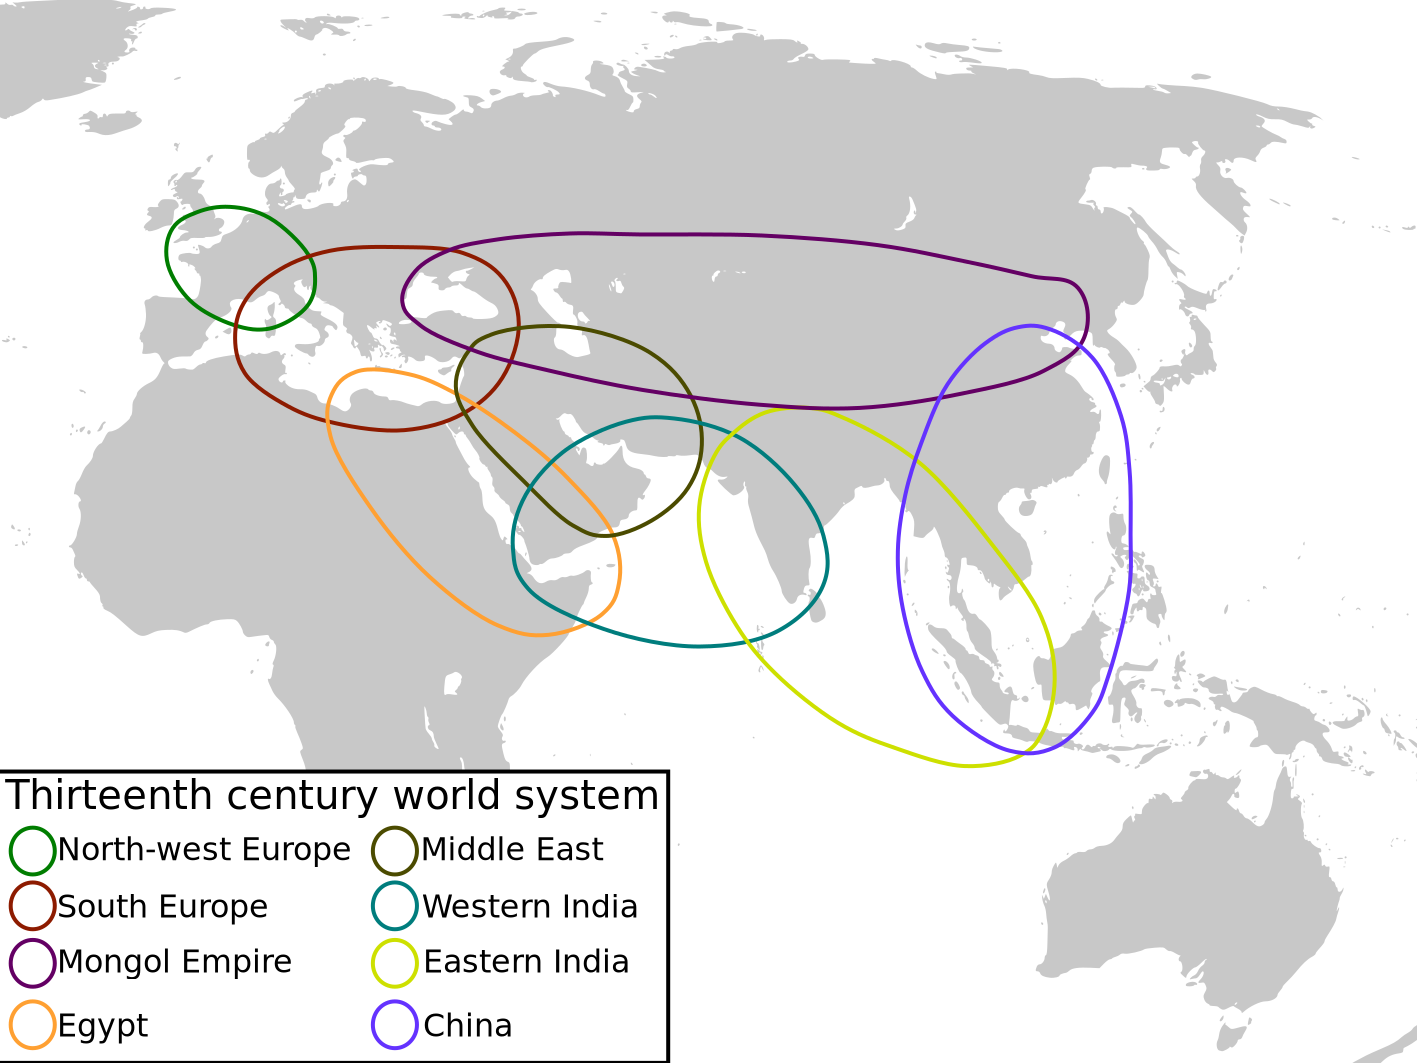
\includegraphics[scale=0.25]{fig1.png}
    \caption{The Trade System of the thirteenth century}
    \label{Figure 1}
\end{figure}

In order to retrace the origins of globalization one must first look at the different criteria required for globalization to occur. This phenomenon of increasing links of various types between multiple regions or individuals around the world only needs for there to be multiple civilizations distant from each other that are aware of their existences and are in contact between themselves. These simple criteria were met when the first civilizations emerged. Keeping this in mind, the first cases of globalization would result in trades between Sumer and the Indus Valley Civilization in 3000 BC. It can also be argued that a more advanced form of archaic globalization was birthed during the Hellenistic Age (323 BC to 31 BC). This period saw many trades centered on the Greek culture over a wide range from India to Spain, as well as trades between the Roman and Parthian Empires and the Han Dynasty. The rise of those commercial links prompted the creation of the Silk Road, that extends from eastern China to the boundaries of the Parthian Empire and towards the city of Rome. The next important period for early globalization is the Islamic Golden Age from the eight to the fourteenth century. During this age the Greek, Muslim and Roman empires extended their territories and covered areas such as China and the Middle East. This age also saw major religions like Christianity, Islam and Buddhism spread to foreign lands. It was at this age that the aforementioned Silk Road was thoroughly developed. During the twelfth and thirteenth century was developed an international trade system between countries ranging from northwestern Europe to China. (Figure \ref{Figure 1})

All in all, archaic globalization can be said to consist of three principles : the universalizing of kingship which led soldiers and kings alike to far further distances in search of honor and prestige, and allowed for travelers to trade goods in distant countries and thus increase the amount of social and economical relationships. One of the greatest global movements of people was still pilgrimages, as well as the need of better medicine, which created more trading routes, especially towards China. And despite the trade system implemented during this period, archaic globalization stays limited to the Old World.

\subsection{Proto-Globalization}

The second period of Globalization starts in 1600 and lasts around 200 years. The most noticable change between the archaic and proto-globalization is the evolution of trade systems. During the twelfth and thirteenth centuries most trade items were rare to foreign countries. Europeans would often buy from eastern countries silk, porcelain and spices. With the arrival of proto-globalization, the trade system saw a shift in merchandises, as now most trade items would rather be commodities like rice, cotton and tobacco. This shift helped the development of early capitalism which began in the Atlantic and spread throughout the world by the beginning of the nineteenth century. There are several reasons for this shift in traded goods, the first one being the rise of the slave trade. (to continue)

\subsection{Modern Globalization}

\section{The Impact of Globalization on the Economy}
The global economy is now a denser network than ever before. Between 1950 and 2010, World merchandise trade – measured by exports-increased by about thirty-three times, while world gross domestic product increased by about nine times over the same period. This phenomenon can also be observed at the country level, in different proportions and at different times. It reflects the increased specialization and division of value-added chains of enterprises and industries, as well as the integration of many countries into the global economy. The World Trade Organization (WTO) includes 157 countries, a number more than ever. Globalization also affects trade in services and trade in capital, labor and know-how. It can be observed that globalization has continued to make strong progress in recent decades, both for commodity flows and – particularly in Switzerland-for the exchange of factors of production. The causes of this progression are many. They are first of all technological in nature: means of transport, such as ships, aircraft and trucks, have improved their performance. The evolution of communication technologies - from the Telegraph to the internet via telephone and fax-has also played an important role in the growth of global trade. The exchange of inputs has also benefited from numerous institutional improvements, notably in the area of legal security, financial architecture and social insurances. The political dimension cannot be underestimated. The impact of the two world wars and the accompanying restrictions on trade was such that globalization, which had reached a very high level before 1914, collapsed. It was only around 1980 that the share of exports and imports in GDP exceeded that achieved before the First World War. The numerous rounds of negotiations under the General Agreement on Tariffs and trade (Gatt) since 1948 and the founding of the WTO in 1995 have reduced trade barriers on a global scale and prevented them from being strengthened during the recent economic and financial crisis. The removal of barriers to capital transfers and the facilitation of migration.

\subsection{The positive effects of Globalisation}

What effect has this tremendous growth in economic interdependence had on global growth and prosperity? Theoretical and empirical research here agree on a surprisingly clear answer: the opening up of markets, through the liberalization of trade in goods, services and factors of production - such as labor, capital and know-how promotes growth and leads to greater macroeconomic prosperity. This statement is supported by the results of various research. Wacziarg and Welch (2008), who examined the effects of trade liberalization on economic growth, show that open countries are growing faster than closed countries. These authors found that states that liberalized their foreign trade between 1950 and 1998 had an average economic growth of 1.5 per cent higher than others. The research of Wacziarg and Welch thus confirms the essential contributions of the classical theses of Sachs and Warner (1995). The same authors have also shown that open national economies converge towards the same level of income. In this group, poor countries grow significantly faster than rich ones, while in closed national economies, no systematic gap in growth between rich and poor countries can be observed. Openness therefore benefits poor countries in particular. This positive effect of openness is particularly evident when a country turns to World Trade in a relatively short time, as many Asian countries have done. China and Vietnam, for example, after opening up by political decision, have experienced very strong growth. Now here is the contrast between openness and autarchy more evident than on the Korean Peninsula. On the 38th parallel, one of the richest countries and one of the poorest countries on the planet are currently living side by side, despite the fact that the two Korea's had an almost similar history until 1945, that they were barely geographically, linguistically and culturally distinguished, and that they had a similar degree of economic development until the 1960s. Since South Korea opened in the mid-sixties, it has achieved record growth rates. Its northern neighbor, on the contrary, suffers from a near-permanent famine.

\begin{figure}[h]
    \centering
    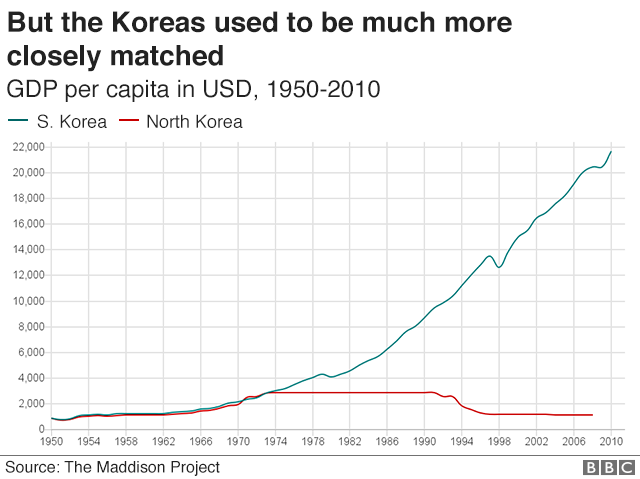
\includegraphics[scale=0.7]{korea.png}
    \caption{GDP per capita comparison between the two Korea}
    \label{Figure X}
\end{figure}

\subsection{Channels of Influence}

International trade theory identifies different channels through which international trade influences prosperity and growth. The work of David Ricardo was decisive in this regard: in 1817, in the chapter "foreign trade" of his book the principles of political economy and taxation, he showed that countries increase their prosperity by specializing in areas where they are more competent than others. This highlighting of comparative advantages implies that a country, while having limited resources, can increase its overall consumption, and that it needs to use fewer resources to achieve a certain level of consumption. The adjustment of wages within a country's economy ensures that, regardless of its productivity, it can participate in international trade. The absolute advantages of a country in a given industry are not taken into account. Trade is not conducive to prosperity because it creates jobs, for example, but because the goods produced increase imports and make more efficient use of limited resources. The classical theory has been enriched in almost two hundred years by very many teachings. While Ricardo linked the comparative advantages of countries to technological gaps, Heckscher and Ohlin's neoclassical theory of trade focused in the first half of the twentieth century on differences in access to resources and factors. This new approach has led to interesting discoveries about the adjustment of factor prices – e.g. wages-between different countries. About 30 years ago, another theory, closely related to the name of Paul Krugman, appeared, called the new theory of trade, which mainly places the advantages of it in the expansion of markets and in the consequent possibility for companies to create their products with less resources. This research focus, which is still very active today, also focuses on increased competition and its effects on the development of firms at different levels of productivity. The channels of influence thus identified relate not only to trade in goods and services but also apply similarly to the exchange of inputs and intermediate products. In all these areas, trade means that resources are used where they make the best contribution to value added. In addition to these so-called allocation effects, which allow for a single increase in prosperity, there are longer-term effects on growth. Trade and direct investment promote the diffusion of technologies at the international level, enabling less developed countries to increase their production by using technologies without having to carry out the necessary research. This partly explains the fact that China has been growing faster for decades than Western countries have experienced in their history.

\subsection{Reverse of the medal}

So, if globalization is so positive, why is it struggling to convince today? At least two reasons can be advanced. First, it does not necessarily benefit everyone in the same country; some may also suffer. Secondly, it can exacerbate environmental damage when institutions are insufficiently equipped. The first aspect refers to the Stolper-Samuelson theorem (1941), generalized by Jones (1965) under the concept of "Magnification Effect", according to which globalization leads to a sharp change in the relative prices of factors in the countries concerned. The relative decline in incomes of low-skilled labor observed in several countries could thus be linked to progress in international trade. Another explanation lies in technological progress, which replaces low-skilled labor with capital. In the case of Switzerland, the relative wages of the low-skilled labor force do not decrease, but its relative unemployment increases. However, as  Weder and Wyss (2011) show, this phenomenon cannot be linked to international trade (but possibly to immigration).The increase in inequality that accompanies strong economic growth in countries such as China or India is not unusual, it is similar to that experienced by European countries in the nineteenth century. The increase in inequality in China is explained by the fact that cities are enriching at a rapid rate and that agricultural regions cannot keep up. However, it would be wrong to say that the poor in China do not benefit from the country's rise. Dollar and Kraay (2004) have shown in an empirical study involving more than one hundred countries that commodity trade liberalization has a positive effect on poverty reduction within countries. The second aspect relates to the negative effects that globalization can have on environmental pollution and overexploitation of resources. Certain types of pollutants-such as those generated by transport in particular – are undoubtedly directly related to increased trade. The main environmental consequences of globalization are, however, linked to the parallel increase in prosperity. Theoretical and empirical analyses of this complex relationship identify varied effects on pollution, some of which are neutralized. Antweiler, Copeland and Taylor (2001) thus show that, while trade leads to increased production and thus pollution (scale effect), increased incomes at the same time lead States to tighten their environmental guidelines, forcing companies to implement more sophisticated environmental techniques (technical effect). In their study, which addresses sulfur dioxide (SO2) emissions in many countries, it is the second effect that prevails; thus, trade reduces pollution. For other substances – however, such as carbon dioxide (CO2), the first effect appears to prevail (Cole and Elliott, 2003). The impact of trade on the environment is therefore highly dependent on the type of pollution and state countermeasures. While for SO2, the state and the economy have supported measures to improve production techniques, for CO2 the willingness to reduce emissions seems much weaker. Neglecting environmental issues leads to the emergence of ill-anticipated externalities. In such a case, international trade can strengthen those that are undesirable. For example, as Taylor (2011) learns, the gigantic, unprotected bison hordes that roamed the central United States were virtually wiped out in the space of fifteen years towards the end of the 19th century following the discovery in Europe of a technique that made industrial exploitation of bison skins possible. Without the existence of trade between Europe and the United States, such unrestrained exploitation would not have taken place, at least to such an extent and at such a rate; this, of course, would not have been the case if the state had ensured their protection.

\subsection{Closure}

Globalization thus has a positive effect on growth and prosperity. It also tends to reduce poverty, even if it risks increasing inequalities within a country. International trade can also have a positive effect on the environment, as prosperity helps, environmental regulations tend to harden. Ecology and resources are particularly at risk of disasters when trade leads to rapid and uncontrolled over-exploitation of (global) common goods. Policies must then act by taking targeted measures: protecting, for example, a species or levying a CO2 tax.

\section{Bibliography}

\subsection{Articles and Websites}
\begin{itemize}
    \item Wikipedia, Globalization
    \item Wikipedia, History of Globalization
    \item Wikipedia, Archaic Globalization
    \item Wikipedia, Proto-globalization
    \item VOX, \textit{Eighteenth-century "proto-globalisation"}, by Paul Sharp
\end{itemize}

\listoffigures

\end{document}
